%%── PANEL 4: Temas 1 y 2 ────────────────────────────────────────────────────
\panel{LightBg}{%
  \phdr{Navy}{1 · Introducci\'on a la Teor\'ia de Ramsey}
  {\scriptsize La Teor\'ia de Ramsey estudia cu\'ando una estructura
  suficientemente grande contiene \emph{siempre} cierta subestructura
  ordenada.}
  \vspace{2pt}

  \begin{tcolorbox}[key]
    {\scriptsize\bfseries Principio del palomar:}
    {\scriptsize $n{+}1$ objetos en $n$ cajones $\Rightarrow$
    alg\'un caj\'on tiene $\geq 2$.}
  \end{tcolorbox}

  \begin{tcolorbox}[def,title={N\'umero de Ramsey $R(s,t)$}]
    {\scriptsize M\'inimo $n$ tal que toda 2-coloraci\'on de aristas de
    $K_n$ contiene un clique \textcolor{blue!70!black}{\bfseries azul}
    de tama\~no $s$ \textbf{o} uno \textcolor{red!70!black}{\bfseries rojo}
    de tama\~no $t$.}
  \end{tcolorbox}

  \begin{tcolorbox}[key]
    {\scriptsize $R(3,3)=6$ \quad $R(3,4)=9$ \quad $R(4,4)=18$}
  \end{tcolorbox}

  \phdr{Navy}{2 · El problema de la amistad}
  {\scriptsize En un grupo de 6 personas, \textbf{?`}siempre existen 3 que
  se conocen o 3 que se desconocen? Se modela como $K_6$: aristas
  \textcolor{red!70!black}{\bfseries rojas} = conocidos,
  \textcolor{blue!70!black}{\bfseries azules} = desconocidos.}

  \begin{center}
  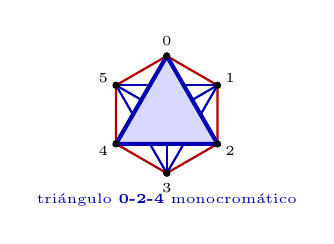
\begin{tikzpicture}[scale=0.62]
    \foreach \i/\ang in {0/90,1/30,2/-30,3/-90,4/-150,5/150}
      \coordinate (v\i) at (\ang:1.2cm);
    \draw[red!70!black,thick] (v0)--(v1)--(v2)--(v3)--(v4)--(v5)--cycle;
    \foreach \i/\j in {0/2,0/3,0/4,1/3,1/4,1/5,2/4,2/5,3/5}
      \draw[blue!70!black,thick] (v\i)--(v\j);
    \fill[blue!15] (v0)--(v2)--(v4)--cycle;
    \draw[blue!70!black,line width=1.5pt] (v0)--(v2)--(v4)--cycle;
    \foreach \i/\ang in {0/90,1/30,2/-30,3/-90,4/-150,5/150}{
      \filldraw[black] (v\i) circle (1.8pt);
      \node[font=\tiny] at (\ang:1.50cm) {$\i$};
    }
    \node[font=\tiny,blue!70!black] at (0,-1.75cm)
      {tri\'angulo \textbf{0-2-4} monocrom\'atico};
  \end{tikzpicture}
  \end{center}

  {\scriptsize\textbf{Prueba:} $v$ tiene 5 aristas; $\geq 3$ del mismo color.
  Si 3 son rojas a $u_1,u_2,u_3$: si $u_iu_j$ rojo $\Rightarrow$ tri\'angulo
  rojo; si todos azules $\Rightarrow$ tri\'angulo azul. $\square$}
}%
